\documentclass{lab_sheet}
\usepackage{epstopdf}
\begin{document}
    \titlePage{Signal Analysis using MATLAB}{March 1, 2021}
    \section{Some MATLAB Commands}
  \begin{table}[H]
    \centering
    \begin{tabular}{||C{3cm}||C{4cm}||C{7.5cm}||}
        \toprule
        \textbf{Command}& \textbf{General Description} & \textbf{Argument Description}\\
        \midrule
        \midrule
        hold & Retain current plot when adding new plots.  & \begin{itemize}
            \item $hold$ $on$: Retains plots in the current axes. 
            \item $hold$ $off$: Sets the hold state to off so that new plots added to the axes clear existing.
        \end{itemize}
        \\
        \hline
        plot    & Creates a 2-D line plot.                    & $plot(X,Y)$: Plot data in Y versus the corresponding values in X.                                                                                                                                      \\ \hline
    subplot & Create axes in tiled positions.             & $subplot(m,n,p)$: Divides the current figure into an m-by-n grid and creates axes in the position specified by p.                                                                                      \\ \hline
    stem    & Plot discrete sequence data                 &  $stem(Y)$: Plots the data sequence, Y, as stems that extend from a baseline along the x-axis.                                                                                                         \\ \hline
    title   & Add title                                   & $title(titletext)$: Uses titletext as the title string for the current axes or standalone visualization.                                                                                                            \\ \hline
    xlabel  & Label for X-axis.                           & $xlabel(text)$: Uses text as the xlabel string.                                                                                                                                                                \\ \hline
    ylabel  & Label for Y-axis.                           & $ylabel(text)$: Uses text as the ylabel string.                                                                                                                                                                \\ \hline
    input   & Request user input.                         & $input(prompt)$: Displays the text in prompt and waits for the user to input a value.                                                                                                                  \\ \hline
    sin     & Sine of argument in radians.                & $sin(X)$: Sine of X.                                                                                                                                                                                  \\ \hline
    cos     & Cosine of argument in radians.              & $cos(X)$: Cosine of X.                                                                                                                                                                                 \\ \hline
    power   & Element-wise power.                         & $power(A,B)$: Raises each element of A to the corresponding powers in B.                                                                                                                               \\ \hline
    conv    & Convolution and polynomial multiplication.  & $conv(u,v)$: Returns the convolution of u and v.                                                                                                                                                       \\ \hline
    fft     & Fast Fourier transform.                     & $fft(X)$: computes the discrete Fourier transform (DFT) of X using a fast Fourier transform (FFT) algorithm.                                                                                           \\ \hline
    freqz   & Frequency response of digital filter.       & $[h,w] = freqz(b,a,n)$: Returns the n-point frequency response vector h and the corresponding angular frequency vector w for the digital filter with transfer function coefficients stored in b and a. \\ \hline
    abs     & Absolute value and complex magnitude.       & $abs(X)$: Returns the absolute value of each element in array X. If X is complex, it returns the complex magnitude.                                                                                \\ \hline
    angle   & Phase angle.                                & $angle(z)$: Returns the phase angle in the interval $[-\pi,\pi]$ for each element of a complex array z.          
    \\                                                                                             
        \bottomrule
        \end{tabular}
        \label{tbl:matlab_commands}
        \caption{Some MATLAB commands used during the lab experiment}
  \end{table}
    \section{Basic Signal Visualization}
    In simple terms, signal is a set of data or information such that they represent the behavior of certain phenomena as a function of one or multiple independent variables. A signal is simply the dependent variable changing as a function of independent variable.
    \subsection*{Analog/Continuous Signal}
    If the independent variable attains continuous values, then the signal is called analog/continuous signal. Throughout our course, analog signals have been regarded as function of time, but they aren't limited to this. In general, they are denoted as $x(t)$, $y(t)$, $h(t)$, and so on such that time ($t$) is the independent variable and the signals are a function of $t$. 
    \subsection*{Digital/Discrete Signal}
    If the independent variable attains only discrete values, then the signal is called digital/discrete signal. Discrete signals are represented as a function of an integer number, say $n$. In general, they are denoted as, $x[n]$, $y[n]$, $h[n]$, and so on such that $n$ is the independent variable and the signals are a function of $n$.
    \subsection{Sinosoidal Signal}
    The sine and cosine signals were plotted in the same co-ordinate axes. This kind of visualization is key to compare signals and their behaviors. The sin and cos functions in MATLAB return the corresponding sine and cosine values for the input argument. The use of hold state allows the figure to retain the previous plots.
    \matlabcode{sinosoidal}{visualization of continuous time signals $x(t)=sin(t)$ and $y(t)=cos(t)$}
    \begin{figure}[H]
        \centering
        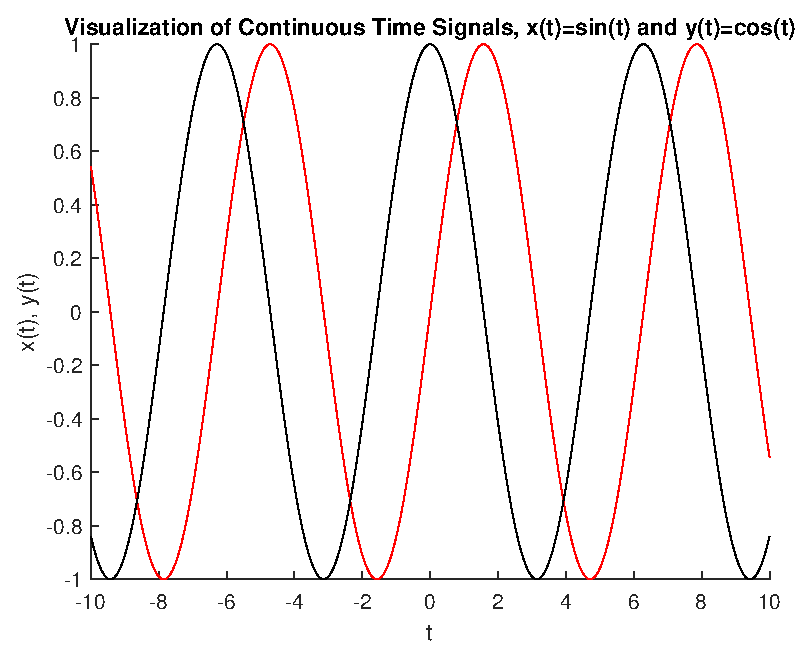
\includegraphics[scale=0.6]{./Figures/sinosoidal}
        \label{fig:sinosoidal}
        \caption{Obtained plot for $x(t)=sin(t)$ and $y(t)=cos(t)$}
    \end{figure}

    \subsection{Ramp Signal}
    Continuous time ramp signal $y(t)=mt$ and discrete time ramp signal $y[n]=mn$ were visualized using MATLAB. The value of $m$ is taken as user input using the input command. The value of $m$ during the execution was selected as 2. The stem function allows us to plot discrete time signals in MATLAB.
    \matlabcode{ramp}{visualization of continuous time $y(t)=mt$ and discrete time $y[n]=mn$ ramp signals}
    \begin{figure}[H]
        \centering
        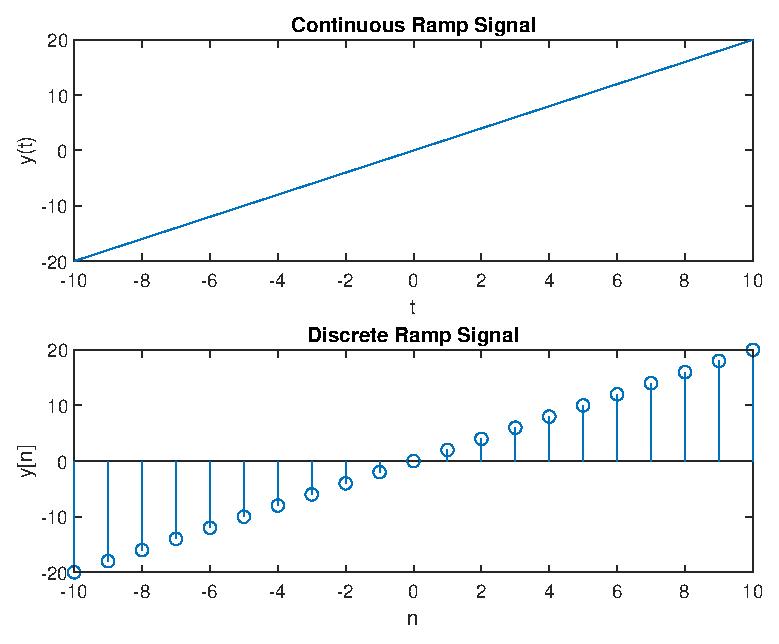
\includegraphics[scale=0.6]{./Figures/ramp}
        \label{fig:ramp}
        \caption{Obtained plot for $y(t)=mt$ and $y[n]=mn$ for $m=2$}
    \end{figure}
    
    \subsection{Exponential Signal}
    Continuous time exponential signal $y(t)=ca^t$ and discrete time exponential signal $y[n]=ca^n$ were visualized using MATLAB. The values of $c$ and $a$ were taken as user input.
    \matlabcode{powered}{visualization of continuous time $y(t)=ca^t$ and discrete time $y[n]=ca^n$ exponential signals}
    \begin{figure}[H]
        \centering
        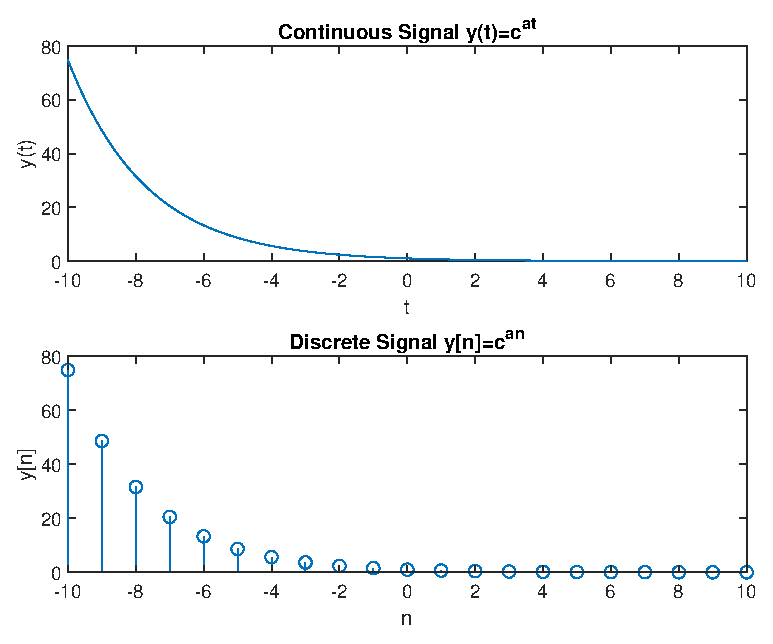
\includegraphics[scale=0.6]{./Figures/powered_1}
        \label{fig:power1}
        \caption{Obtained plot for $y(t)=ca^t$ and $y[n]=ca^n$ for $c=0.75$ and $a=1.5$}
    \end{figure}

    \begin{figure}[H]
        \centering
        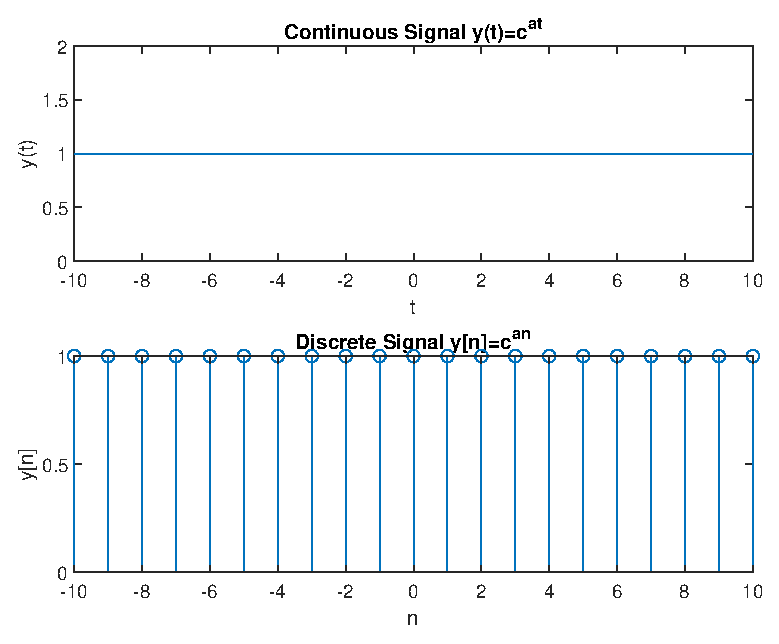
\includegraphics[scale=0.6]{./Figures/powered_3}
        \label{fig:power3}
        \caption{Obtained plot for $y(t)=ca^t$ and $y[n]=ca^n$ for $c=0.75$ and $a=0$}
    \end{figure}

    \begin{figure}[H]
        \centering
        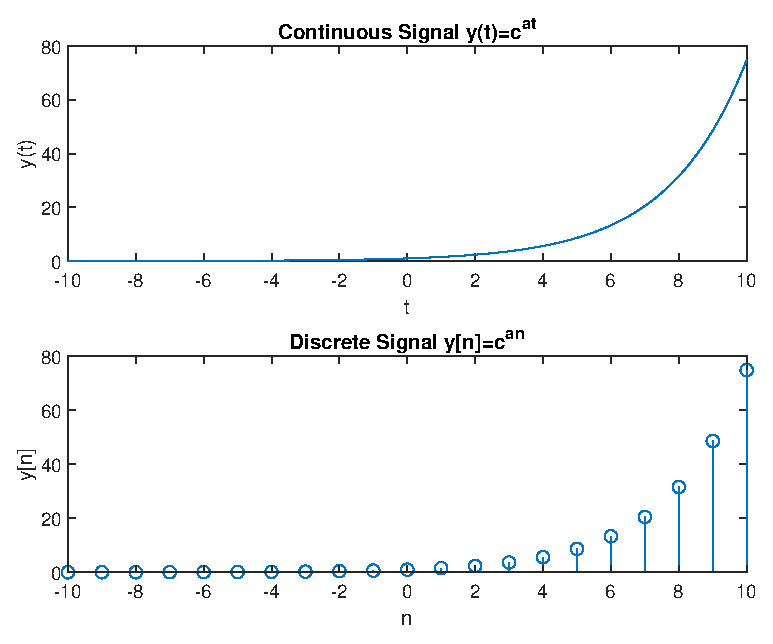
\includegraphics[scale=0.6]{./Figures/powered_2}
        \label{fig:power2}
        \caption{Obtained plot for $y(t)=ca^t$ and $y[n]=ca^n$ for $c=0.75$ and $a=-1.5$}
    \end{figure}

    Likewise continuous time exponential signal $y(t)=ce^{at}$ and discrete time exponential signal $y[n]=ce^{an}$ were visualized using MATLAB. The values of $c$ and $a$ were taken as user input.
    \matlabcode{exp_signal}{visualization of continuous time $y(t)=ce^{at}$ and discrete time $y[n]=ce^{an}$ exponential signals}
    \begin{figure}[H]
        \centering
        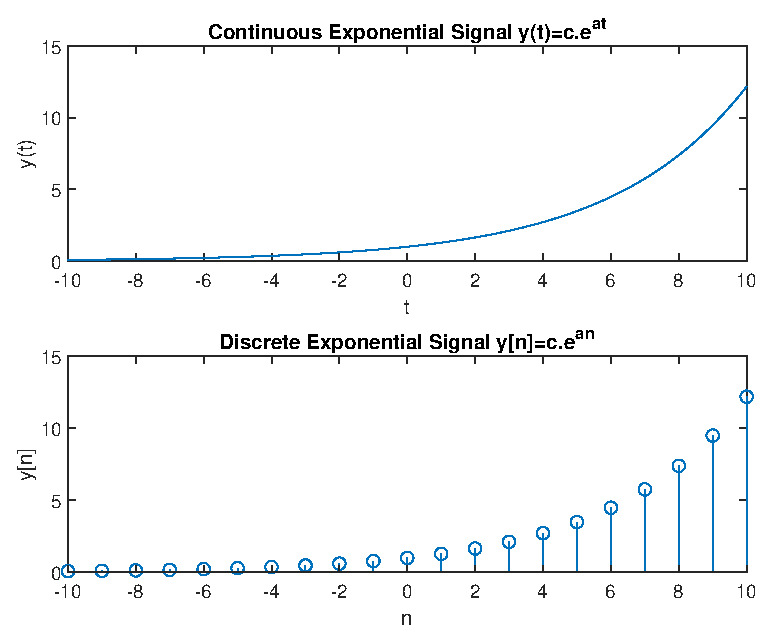
\includegraphics[scale=0.6]{./Figures/exp_signal_1}
        \label{fig:exp1}
        \caption{Obtained plot for $y(t)=ce^{at}$ and $y[n]=ce^{an}$ for $c=1$ and $a=0.25$}
    \end{figure}

    \begin{figure}[H]
        \centering
        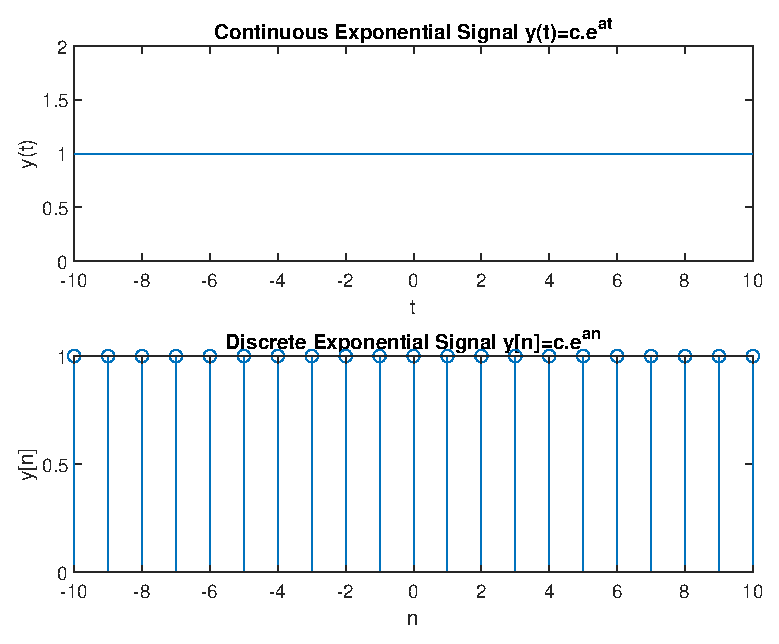
\includegraphics[scale=0.6]{./Figures/exp_signal_2}
        \label{fig:exp2}
        \caption{Obtained plot for $y(t)=ce^{at}$ and $y[n]=ce^{an}$ for $c=1$ and $a=0$}
    \end{figure}

    \begin{figure}[H]
        \centering
        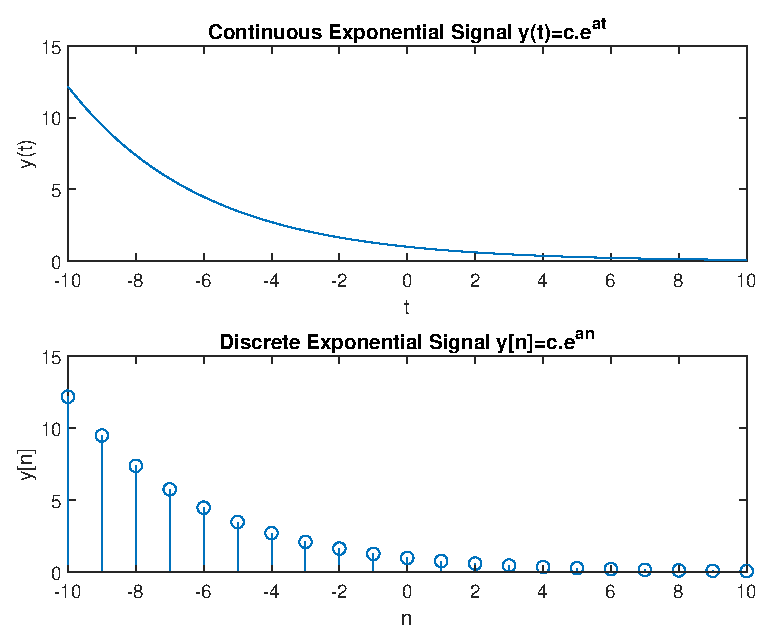
\includegraphics[scale=0.6]{./Figures/exp_signal_3}
        \label{fig:exp3}
        \caption{Obtained plot for $y(t)=ce^{at}$ and $y[n]=ce^{an}$ for $c=1$ and $a=-0.25$}
    \end{figure}

    \subsection{Unit Step Signal}
    Continuous time unit step signal $y(t)= u(t)$ and discrete time ramp signal $y[n]=u[n]$ were visualized using MATLAB. It takes a value 1 for $t>=0$ or $n>=0$ and 0 otherwise.
    \matlabcode{unit_step}{visualization of continuous time $y(t)=u(t)$ and discrete time $y[n]=u[n]$ unit step signals}
    \begin{figure}[H]
        \centering
        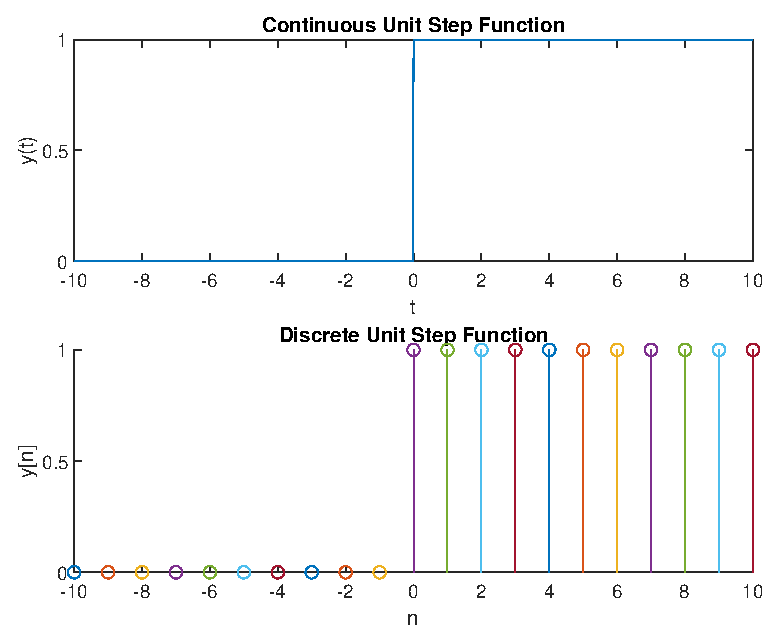
\includegraphics[scale=0.6]{./Figures/unit_step}
        \label{fig:unit_step}
        \caption{Obtained plot for $y(t)=u(t)$ and $y[n]=u[n]$}
    \end{figure}

    \subsection{Unit Impulse Signal}
    Continuous time unit step signal $y(t)= \delta(t)$ and discrete time ramp signal $y[n]=\delta[n]$ were visualized using MATLAB. It takes a value 1 for $t=0$ or $n=0$ and 0 otherwise.
    \matlabcode{unit_impulse}{visualization of continuous time $y(t)=\delta(t)$ and discrete time $y[n]=\delta[n]$ unit step signals}
    \begin{figure}[H]
        \centering
        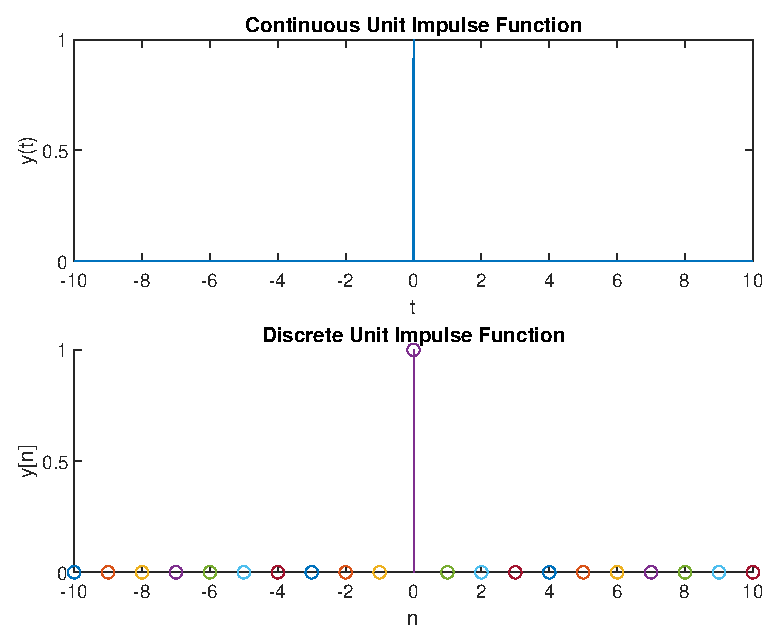
\includegraphics[scale=0.6]{./Figures/unit_impulse}
        \label{fig:unit_impulse}
        \caption{Obtained plot for $y(t)=\delta(t)$ and $y[n]=\delta[n]$}
    \end{figure}

    \section{Fourier Series}
    For a periodic continuous time signal $x(t)$ with $T$ period, the fourier series representation is,
    $$
    x(t)=\sum_{k=-\infty}^{\infty}a_k e^{jk\omega_0 t}
    $$
    such that $\omega_0 = \frac{2\pi}{T}$ and the fourier coefficients are given as,
    $$
    a_k = \int_T x(t) e^{-j \omega_0 t}dt
    $$
    Likewise, the fourier series representation of a square wave with period $T$ and amplitude $a$ is mathematically given as,
    $$
    x(t)=\frac{4a}{\pi} \sum_{k=1}^{\infty}\frac{sin((2k-1)\omega_0 t)}{2k-1}
    $$
    The sum of all the odd harmonics of the sinosoidal signal forms a square wave approximation.
    \matlabcode{sin_odd_add}{fourier series representation of a square wave}
        \begin{figure}[H]
        \centering
        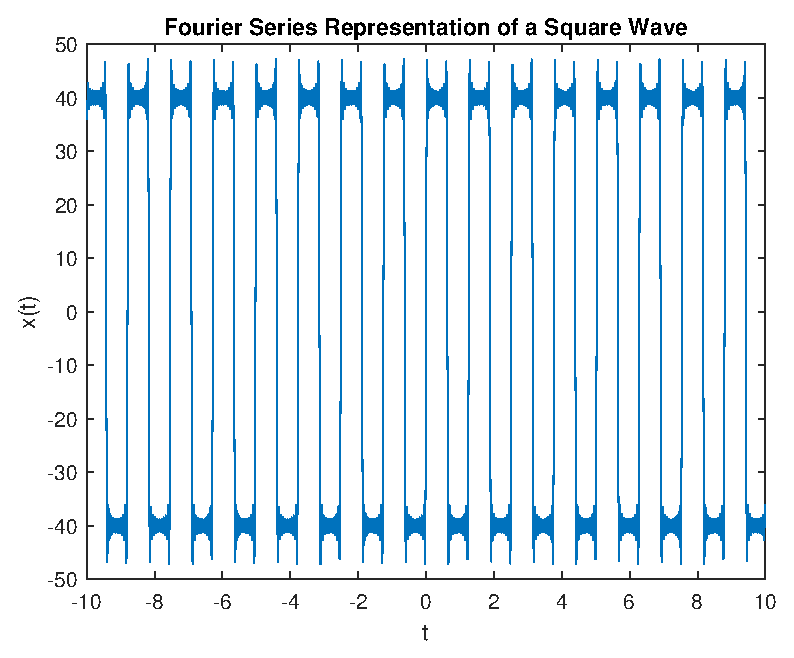
\includegraphics[scale=0.7]{./Figures/sin_add_odd_1}
        \label{fig:sin1}
        \caption{Obtained plot for fourier series of $x(t)$ with first 20 terms}
    \end{figure}

    \begin{figure}[H]
        \centering
        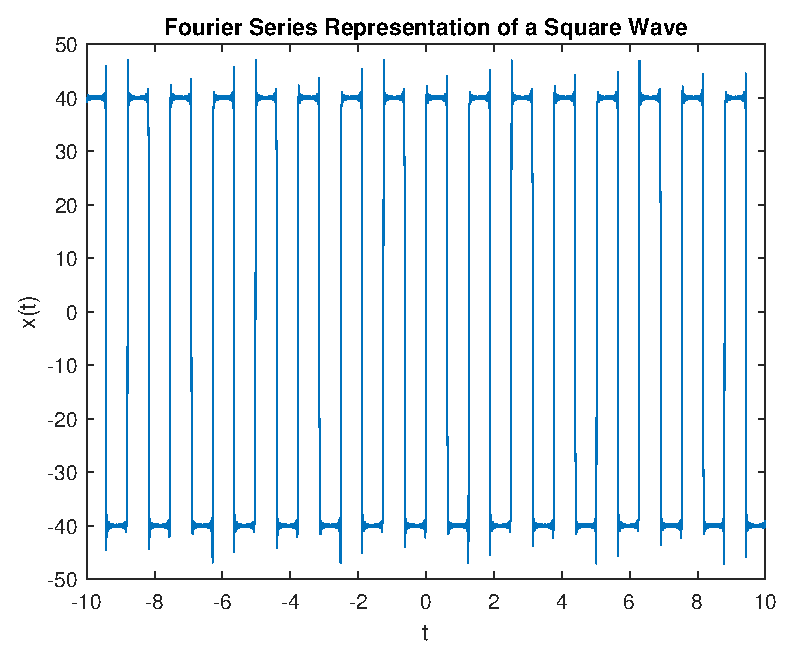
\includegraphics[scale=0.7]{./Figures/sin_add_odd_2}
        \label{fig:sin2}
        \caption{Obtained plot for fourier series of $x(t)$ with first 100 terms}
    \end{figure}

    \begin{figure}[H]
        \centering
        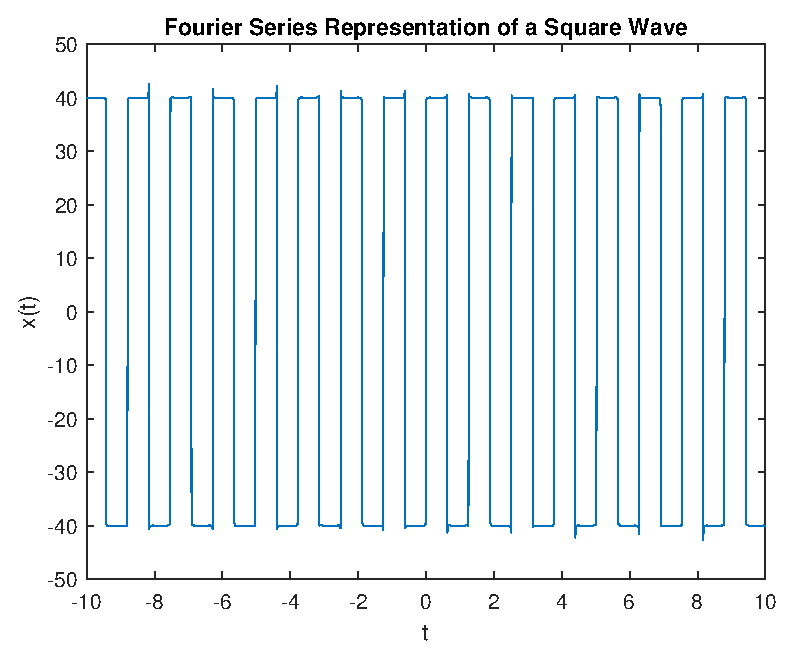
\includegraphics[scale=0.7]{./Figures/sin_add_odd_3}
        \label{fig:sin3}
        \caption{Obtained plot for fourier series of $x(t)$ with first 1000 terms}
    \end{figure}
    With the increase in number of terms used, the ripples also increases based on the Gibbs phenomenon.

    \section{Convolution}
    The convolution of two continuous time signals $x(t)$ and $h(t)$, called the convolution integral, is mathematically given as,
    $$
    y(t)=x(t)*h(t)=\int_{-\infty}^{\infty}x(u)h(t-u)du
    $$
    Likewise, the convolution of two discrete time signals $x[n]$ and $h[n]$, called the convolution sum, is mathematically given as,

    $$
    y[n]=x[n]*h[n]=\sum_{k=-\infty}^{\infty} x[n]h[n-k]
    $$
    The conv function returns the convolution for two discrete sequences in MATLAB.
    \matlabcode{dis_convo}{convolution for two discrete sequences $x[n]=[1,3,2,1,1]$ and $h[n]=[1,2,-1,1]$}
    \begin{figure}[H]
        \centering
        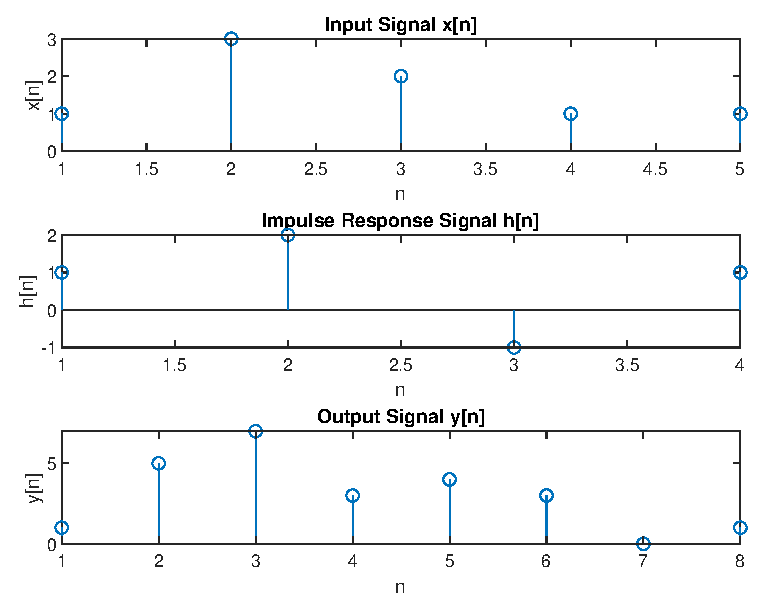
\includegraphics[scale=0.6]{./Figures/dis_convo}
        \label{fig:conv}
        \caption{Obtained plot for convolution of $x[n]=[1,3,2,1,1]$ and $h[n]=[1,2,-1,1]$}
    \end{figure}

    \matlabcode{dis_convo_2}{convolution for two discrete sequences $x[n]=0.5^n$ and $h[n]=u[n]$}
    \begin{figure}[H]
        \centering
        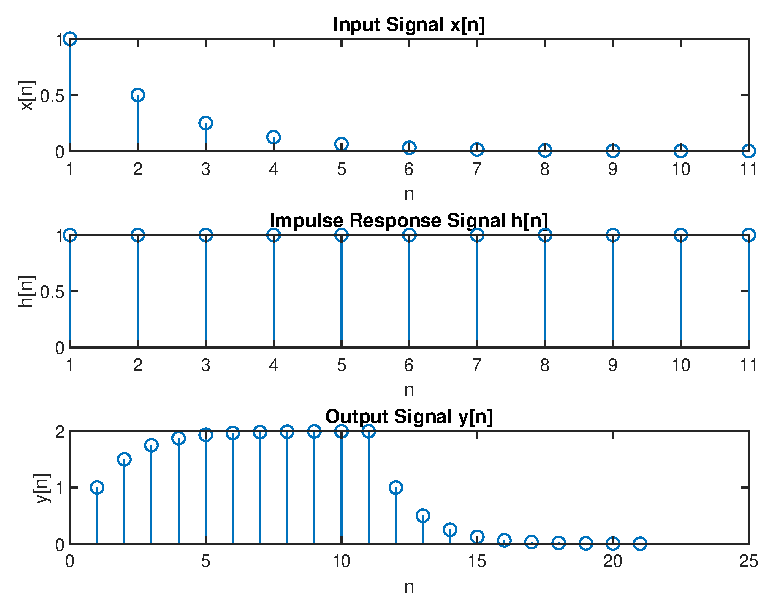
\includegraphics[scale=0.6]{./Figures/dis_convo_2}
        \label{fig:conv2}
        \caption{Obtained plot for convolution of $x[n]=0.5^n$ and $h[n]=u[n]$}
    \end{figure}

    \section{Fourier Transform}
    The fourier transform of a continuous time signal $x(t)$ is mathematically given as,
    $$
    X(j\omega) = \int_{-\infty}^{\infty} x(t) e^{-j\omega t} dt
    $$
    Likewise, the fourier transform of a discrete time signal $x[n]$ is mathematically given as,
    $$
    X(e^{j\omega})=\sum_{n=-\infty}^{\infty} x[n] e^{-j\omega n}
    $$
    The fft function returns the real and imaginary parts of the fast fourier transform for the input argument. The real and imaginary parts are plotted separately.

    \matlabcode{fourier_transform}{fourier transform of discrete sequence $x[n]=[0,1,2,3]$}
    \begin{figure}[H]
        \centering
        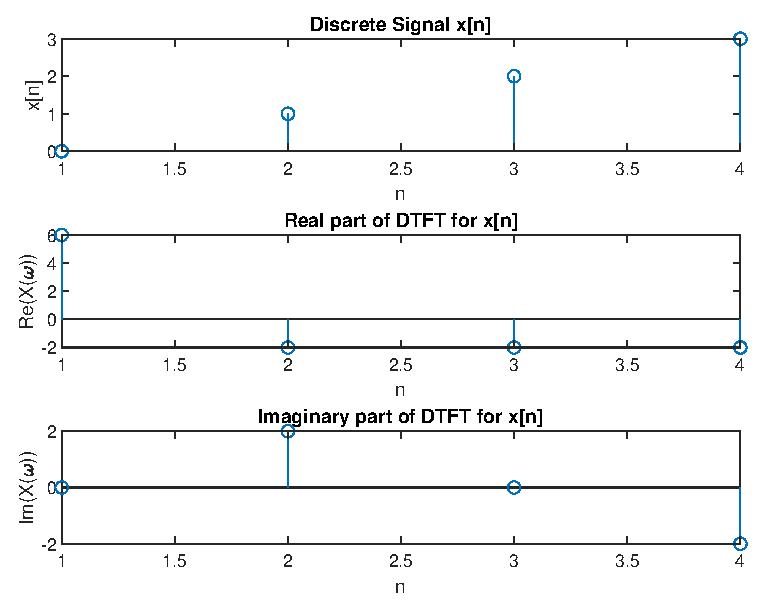
\includegraphics[scale=0.6]{./Figures/fourier_transform}
        \label{fig:fourier}
        \caption{Obtained plot for fourier transform of $x[n]=[0,1,2,3]$}
    \end{figure}

    \section{Frequency Response of a System}
    For a system with $h(t)$ as the impulse response, and $x(t)$ as the input signal, the output $y(t)$ is related to the input as the convolution,
    $$
    y(t)=x(t)*h(t)=\int_{-\infty}^{\infty}x(u)h(t-u)du
    $$
    According to the convolution property of fourier transforms, the fourier transforms of the signals are related as,
    $$
    Y(j\omega)=H(j\omega)X(j\omega)
    $$
    where $H(j\omega)$, the fourier transform of the impulse response of the system is the frequency response of the system. Likewise, for discrete time input signal $x[n]$ to a system with the impulse response $h[n]$, the output in frequency domain is mathematically given as,
    $$
    Y(e^{j\omega})=H(e^{j\omega})X(e^{j\omega})
    $$
    where $H(e^{j\omega})$, the fourier transform of the impulse response of the system is the frequency response of the system.
    During the lab experiment, we plotted the frequency response given as,
    $$
    H(z)=\frac{0.008-0.033z+0.05z^2-0.033z^3+0.008z^4}{1+2.37z+2.7z^2+1.6z^3+0.5z^4}
    $$
    The freqz function returns the frequency response of a system whose amplitude and phase were plotted separately in MATLAB.

    \matlabcode{freq_response}{plotting frequency response of$H(z)$}
    \begin{figure}[H]
        \centering
        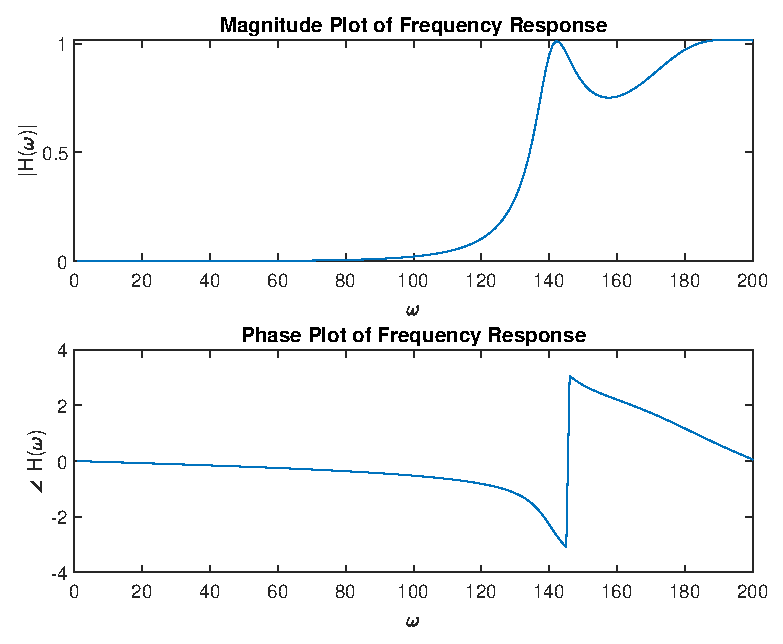
\includegraphics[scale=0.6]{./Figures/freq_response}
        \label{fig:fourier}
        \caption{Obtained plot for frequency response of $H(z)$}
    \end{figure}

    \section{Conclusion}
    In this lab experiment, we dealt with the basics of signal analysis using MATLAB. The experiments included visualization of basic signals such as sinosoidal, ramp, exponential, unit step and unit impulse. The fourier series approximation of a square wave was also visualized using sinosoidal signal's odd harmonics. Convolutions of discrete signals were also plotted in MATLAB. Likewise, the fourier transform and frequency response of given signals were plotted using the respective functions. Hence, the overall objectives of the lab experiment were fulfilled. 
\end{document}
